\documentclass[9pt,twocolumn]{pnas-new}
\usepackage{supertabular}
\usepackage{lscape}
\usepackage{multirow}
\usepackage{tabularx}
\usepackage{csquotes}
\usepackage{upgreek}
\usepackage{hyperref}
\usepackage{lineno}
\usepackage{rotating}
\usepackage{adjustbox}

%\templatetype{pnasresearcharticle} % Choose template 
%pnasmathematics
\title{Gender stereotypes are reflected in the distributional structure of 25 languages}

% Use letters for affiliations, numbers to show equal authorship (if applicable) and to indicate the corresponding author
\author[a,*]{Molly Lewis}
\author[b]{Gary Lupyan} 

\affil[a]{Carnegie Mellon University, Psychology Department/Social and Decision Sciences, Pittsburgh, PA, USA}
\affil[b]{University of Wisconsin-Madison, Psychology Department, Madison, WI, USA}


\begin{abstract}
Cultural stereotypes such as the idea that men are more suited for paid work while women for taking care of the home and family may contribute to gender imbalances in science, technology, engineering and mathematics (STEM) fields among other undesirable gender disparities. We examine whether gender stereotypes are reflected in the large-scale distributional structure of natural language semantics. We measure gender associations embedded in the statistics of 25 languages and relate these to data on an international dataset of psychological gender associations (\emph{N} = 656,636). People's implicit gender associations are strongly predicted by gender associations encoded in the statistics of the language they speak. These associations are further related to the extent that languages mark gender in occupation terms (e.g., ``waiter''/``waitress''). Our pattern of findings is consistent with the possibility that linguistic associations shape  people's implicit judgments.

\end{abstract}

\leadauthor{Lewis}

\begin{document}

\maketitle
\thispagestyle{firststyle}
\ifthenelse{\boolean{shortarticle}}{\ifthenelse{\boolean{singlecolumn}}{\abscontentformatted}{\abscontent}}{}


\let\thefootnote\relax\footnotetext{*Corresponding author: Molly Lewis (mollylewis@cmu.edu)}

By the time they are two, children  have begun to acquire the
gender stereotypes in their culture (1). These
stereotypes can have undesirable effects. For example, in one study,
6-year-old girls were less likely than boys to choose activities that
were described as for children \enquote{who are very, very smart} and
also less likely to think of themselves as \enquote{brilliant}  (2). Such beliefs may, over time, translate to the observed lower rates of female participation in science, technology, engineering and mathematics (STEM) fields (3-6) and are reflected in large differences in perceived self-efficacy; boys reported having greater ability to understand and explain various scientific findings  (independent of actual ability,6).  Here we attempt to understand where such beliefs may come from.

We can distinguish between two major sources of information that contribute to gender stereotypes. The first is direct experience. For
example, one may observe that most nurses are women and most
philosophers are men and conclude that women are better suited for
nursing and men for philosophy. The second is language. Even without any
direct experience with nurses or philosophers, one may learn about their
stereotypical gender from language about nurses and philosophers.
Languages encode gender in multiple ways. These include gender-specific
titles (\enquote{Mr.} vs.\ \enquote{Miss.}), proper names (\enquote{Sam}
vs.\ \enquote{Ashley}), pronouns (\enquote{he} vs.\ \enquote{she}),
certain job titles (\enquote{waiter} vs.\ \enquote{waitress}), and
higher-order linguistic associations (otherwise gender-neutral words can
become gendered by being associated with explicitly gendered contexts).
Another source of linguistic information comes from sex-based
grammatical gender systems found in approximately 30\% of languages (7). For example, in Spanish, the gender of a
nurse must be specified grammatically (\enquote{enfermer\emph{a}} vs.
\enquote{enfermer\emph{o}}).

To the extent that language is a source of information for forming
cultural stereotypes, two people with similar direct experiences, but
different linguistic experiences, may develop different stereotypes.
Some past work hints at people's surprising sensitivity to
stereotype-relevant information delivered through language. Young
children perform worse in a game if they are told that someone of the
opposite gender performed better than they did on a previous round
(8), or merely told that the game is associated
with a particular gender (9). In some
cases, a subtle turn of phrase can influence children's gender-based
generalization (10,11). For example, Cimpian and Markman found that children were more likely to infer that a novel skill is stereotypical of a
gender if the skill is introduced with a generic as opposed to a
non-generic subject (``{[}Girls are/There is a girl who is{]} really
good at a game called ``gorp''''). Such work shows that in certain
experimental settings, language can influence stereotype formation. We ask whether a similar correspondence between language associations and stereotypes exists in a large corpus of naturalistic text and among an international sample of participants. 

A widely used method for quantifying cultural stereotypes at an
individual level is the \emph{Implicit Association Test} (12). Here, we use previously administered IATs designed to measure a particular type of gender
stereotype: A tendency to associate men with careers and women with family
(13, \emph{N} = 657,335). These data span 39 countries, allowing us to assess how group-level implicit gender associations (14-16) vary as a function of language to which participants are exposed. 

To measure cultural stereotypes in language, we use semantic embeddings derived from a distributional semantics model that is trained by predicting words from surrounding words as they occur in a large corpus. The core assumption of these models is that the meaning of a word can be described by the words it co-occurs with---words occurring in similar contexts tend to have similar meanings (17). The word \enquote{dog}, for example, is represented as more similar to \enquote{cat} than to \enquote{banana} because contexts containing \enquote{dog} are more similar to contexts containing \enquote{cat} than to contexts containing \enquote{banana} (18-20). Gender stereotypes can become encoded in the distributional semantics of language because a word like \enquote{woman} may occur in more similar contexts to words like \enquote{home} and \enquote{family} while a word like \enquote{man} in contexts more similar to \enquote{job} and \enquote{money.} Previous work has shown stereotypes like those studied using IATs can be predicted from the distributional statistics of language (co-occurrences, 21-24). This previous work only measured semantic associations in English. Here, we examine gender associations in the distributional semantics of 25 languages and ask whether languages with stronger career-gender associations predict stronger implicit and explicit gender associations in speakers of those languages.

Discovering that gender associations in language are correlated with people’s implicit and explicit gender associations can be interpreted in several ways  (22,25).  One possibility is that some cultures have stronger gender stereotypes and these are reflected in what people talk about. Language, on this view, simply \emph{reflects} pre-existing associations. However, language may not only reflect pre-existing stereotypes, but may also provide a distinct source of information for
learning about them, thereby constituting a causal influence on the associations people learn (26). Another possibility is that a third variable influences both language and psychological associations. The correlational approach of the present work does not allow us to distinguish between these possibilities; our  goal is to establish whether there is in fact a correspondence between psychological and linguistic gender associations. Establishing whether such a correspondence exists is a prerequisite to understanding the underlying causal model.

In Study 1, we examine whether gender associations derived from the distributional structure of different languages predict responses on the IAT. In Study 2, we examine how the psychological
associations measured by the IAT and the linguistic associations we measure relate
to more structural aspects of language: sex-based grammatical gender and
the prevalence of gender-specific occupation terms (e.g.,
\enquote{waiter}/\enquote{waitress}, but
\enquote{teacher}/\enquote{teacher}). Our results suggest that languages that encode gender stereotypes more strongly -- through either distributional semantics or structural features -- tend to have speakers with stronger stereotypical gender associations. 

\section*{A cross cultural dataset assessing gender associations}\label{description-of-cross-cultural-dataset-of-psychological-gender-bias}

To quantify gender associations, we used data from a large-scale administration of an Implicit Association Task (IAT, 12)  by Project Implicit (13, \url{https://implicit.harvard.edu/implicit/}). The IAT measures the strength of respondents' implicit associations between two pairs of concepts (e.g., male-career/female-family vs.~male-family/female-career) accessed via
words (e.g., \enquote{man,} \enquote{business}). The underlying
assumption of the IAT is that words denoting more similar meanings
are easier to pair together compared to words denoting more dissimilar pairs. Meanings are paired in the task by assigning them to the same response
keys in a two-alternative forced-choice categorization task. In the
critical blocks, meanings are assigned to keys in a way that
is either stereotype-congruent (i.e.~Key A = male/career; Key B =
female/family) or stereotype-incongruent (i.e.~Key A = male/family; Key B =
female/career). Participants are then presented with a word related to
one of the four concepts and asked to classify it as quickly as possible
(see Study 1b Methods for list of target words). Slower reaction times
in the stereotype-incongruent blocks relative to the stereotype-congruent blocks are
interpreted as indicating an implicit association between the
corresponding concepts (i.e.~a tendency to associate male with career and
female with family). Our final sample included 657,335 participants from 39 countries, with a
median of 1,145 participants per country.

To quantify the strength of participants’ implicit association as assessed by the IAT we adopt the widely used  \emph{D-score}, which measures the difference between critical blocks for each participant while controlling for individual differences
in response time (27). After completing
the IAT, participants were asked \enquote{How strongly do you associate
the following with males and females?} for both the words
\enquote{career} and \enquote{family.} Participants indicated their
response on a Likert scale ranging from \emph{female} (1) to \emph{male}
(7). An explicit gender-career association score was defined as their Career response minus their Family response such that greater values indicate a greater tendency to associate males with career.

Replicating previous analyses (13), participants tended to implicitly associate men with career and women with family (\emph{D-Score M} = 0.38 {[}0.38, 0.38{]}; \emph{t}(657334) = 878.3, \emph{p} \textless{} .001). Older participants showed greater implicit associations between women-family and men-career  (\emph{r}(657333) = 0.06 {[}0.06, 0.06{]}, \emph{p} \textless{} .001).  The measured associations were stronger for female participants (\emph{M} = 0.41, \emph{SD} = 0.35) than male participants
(\emph{M} = 0.32, \emph{SD} = 0.37; \emph{t}(338217.04) = 96.82, \emph{p} \textless{} .001; \emph{d} = 0.27 {[}0.26, 0.27{]}) and were larger for participants that received the block of trials with stereotype-incongruent mappings first than those who received the stereotype-incongruent mappings second (\emph{M} = -0.09 {[}-0.09, -0.09{]}; \emph{t}(652694.18) = -104.03, \emph{p} \textless{} .001; \emph{d} = -0.26 {[}-0.26, -0.25{]}). 


Because we did not have language information at the participant level, in the remaining analyses we examine the career-gender association and its predictors at the country level. To account for the above-mentioned influences on implicit associations, we calculated a residual implicit association score for each participant, controlling for participant age, participant gender, and block order. We also calculated a residual explicit association score controlling for the same set of variables. We then averaged across participants to estimate the country-level gender association (Implicit: \emph{M} = -0.01; \emph{SD} = 0.03; Explicit: \emph{M} = 0.00; \emph{SD} = 0.18). Implicit gender associations were correlated with explicit gender associations at the level of participants (\emph{r}(645072) = 0.16 {[}0.16, 0.16{]}, \emph{p} \textless{} .001); At the level of countries, this relationship was stronger, though not statistically reliable (\emph{r}(37) = 0.26 {[}-0.07, 0.53{]}, \emph{p} = 0.12). The weak correlation between implicit and explicit measures is consistent with claims that these two measures tap into different cognitive constructs (28).

Do the implicit and explicit associations measured by the Project Implicit
dataset predict any real world outcomes? We compared our residual
country-level implicit and explicit gender associations to a gender equality
metric reported by the United Nations Educational, Scientific and
Cultural Organization (UNESCO) for each country: the percentage of women
among STEM graduates in tertiary education  (5,6).  Consistent with previous research
(Miller et al., 2015), we found that implicit gender association was negatively
correlated with percentage of women in STEM fields: Countries with
weaker associations between men and career tended to have more women in STEM fields (\emph{r}(31) = -0.54 {[}-0.75, -0.24{]}, \emph{p} = 0.001). In contrast, there was no
relationship between the percentage of women in STEM fields and the
explicit gender association measure used by Project Implicit (\emph{r}(31) = 0.14 {[}-0.21, 0.46{]}, \emph{p} = 0.43). In addition, we found a strong correlation between the
median age of each country's population (29) and the residual implicit association (in which participant age
was held constant): Countries with older populations tended to have
larger gender associations (\emph{r}(37) = 0.64 {[}0.4, 0.79{]}, \emph{p} \textless{} .001).


In sum, we replicate previously-reported patterns of gender association in the
gender-career IAT literature, with roughly comparable effect sizes (c.f. 13). We also find that implicit gender associations predict an objective measure of gender equality---female enrollment in STEM fields. In the Discussion, we comment further on our findings that older participants and participants from countries with older populations show stronger implicit gender associations.

\section*{Study 1: Relating associations in distributional semantics and
human
behavior}\label{study-1-relating-gender-biases-in-distributional-semantics-and-human-behavior}

Are participants' gender associations predictable from the language they
speak? Showing that such a relationship exists is the first step to investigating the underlying causal relationships. We begin by validating word embedding measures of
gender association by comparing them to explicit human judgments of word
genderness (Study 1a). We then apply this method to models trained on
text in other languages (Study 1b and 1c). We find that the implicit gender
association of participants in a country is correlated with the gender associations embedded in the statistics of the dominant language spoken in that country.


In Studies 1a-1c we estimate linguistic gender associations using distributional semantics. By attempting to predict the words that surround another word in large corpora, these models   (e.g., 30) are able to learn a vector-based representation for each word that represents its similarity to other words, i.e., a semantic embedding. We can then compute the similarity between two words by taking the distance between their vectors (e.g., cosine of angle). 
We estimated a gender score for each word by measuring the average cosine distance to a standard set of
male \enquote{anchor} words (\enquote{male,} \enquote{man,}
\enquote{he,} \enquote{boy,} \enquote{his,} \enquote{him,}
\enquote{son,} and \enquote{brother}; 13)
and the average cosine similarity to a set of female words
(\enquote{female,} \enquote{woman,} \enquote{she,} \enquote{girl,}
\enquote{hers,} \enquote{her,} \enquote{daughter,} and
\enquote{sister}). We then obtained a gender score for each word by
taking the difference of the similarity estimates (mean female similarity
- mean male similarity), such that larger values indicated a stronger
association with females. We estimated  gender scores for each word from
models pre-trained on two different corpora of English text: subtitles from movies
and TV shows (31,32 and Wikipedia
(33).

Estimates of gender association from the Subtitle corpus (\emph{M} = 0.01;
\emph{SD} = 0.03) and the Wikipedia corpus (\emph{M} = 0; \emph{SD} =
0.03) were highly correlated with each other (\emph{r}(4669) = 0.71 {[}0.7, 0.73{]}, \emph{p} \textless{} .001). Critically, association estimates from both word embedding
models were also highly correlated with human judgements of word gender (the degree to which a word is associated with females versus males; \emph{M} = 4.10; \emph{SD} = 0.92; Subtitle: \emph{r}(4669) = 0.63 {[}0.61, 0.65{]}, \emph{p} \textless{} .001; Wikipedia: \emph{r}(4669) = 0.59 {[}0.57, 0.6{]}, \emph{p} \textless{} .001; Fig. 1). This suggests that the psychological gender association of a word can be reasonably estimated from word embeddings.

Having validated our basic method, we now use it to examine the relationship
between psychological and linguistic associations of men with career and women with family. In Study 1b, we
estimated the magnitude of these associations in the dominant language
spoken in each country represented in the Project Implicit dataset, and
compare this estimate to estimates of psychological career-gender associations from the
Project Implicit participants.



Despite the differences in the specific content conveyed by the
Wikipedia and the Subtitle corpus, the estimated career-gender association for each
language was similar across the two corpora ($M_{diff}$ = 0 {[}-0.17, 0.16{]}; \emph{t}(19) = -0.06, \emph{p} = 0.95; \emph{d} = -0.01 {[}-0.65, 0.63{]}). We next examined the relationship between these
estimates for each language and the mean career-gender association score
for participants from countries where that language was dominant (and,
we assume, was the native language of most of these individuals).
Implicit career-gender association was positively correlated with estimates of
 career-gender association in language from both the Subtitle (\emph{r}(18) = 0.5 {[}0.08, 0.77{]}, \emph{p} = 0.02)
and Wikipedia trained models (\emph{r}(23) = 0.48 {[}0.11, 0.74{]}, \emph{p} = 0.01; Fig.\ 2a;
Table 1 shows the language-level correlations between all variables in
Studies 1b and 2). Linguistic career-gender association was
not correlated with explicit career-gender association (Subtitle: \emph{r}(18) = -0.08 {[}-0.5, 0.38{]}, \emph{p} = 0.74; Wikipedia: \emph{r}(23) = 0.34 {[}-0.06, 0.65{]}, \emph{p} = 0.09). Estimates
of the career-gender association from the Subtitle corpus were correlated with the
objective measure of gender equality and percentage of women in STEM fields
(\emph{r}(16) = -0.55 {[}-0.81, -0.11{]}, \emph{p} = 0.02). This relationship was not reliable
for the Wikipedia corpus (\emph{r}(20) = -0.19 {[}-0.57, 0.25{]}, \emph{p} = 0.4; see SI Sec. 2.4 for correlations controlling for median country age). 




In Study 1c, we conducted a confirmatory, pre-registered analysis of our hypothesis that associations present in language statistics are reflected in the psychological associations of speakers of those languages. We leveraged the Attitudes, Identities, and Individual Differences Study dataset (AIID, 34) containing measures of IAT performance from over 200,000 participants for a wide range of IATs (e.g. career - family, team - individual, etc.). All the tests were conducted using English words and most participants were English speakers. The dataset allowed us to compare associations between participants who spoke two different dialects of English: British and American. For each of the 31 IATs in the sample, we predicted that the degree to which those associations were present in a speaker’s English dialect (British or American) would predict the magnitude of their psychological association, as measured by the IAT.

Figure 2b visualizes the critical interaction term. Behavioral performance on the different IATs was correlated with language statistics. When language statistics predicted that US-English had a greater association, American participants showed a stronger association in the IAT. When language statistics predicted that UK-English had a stronger association, British participants showed a stronger association in the IAT (\(\beta\) = -.05, \emph{SE} = .02, \emph{t} = -2.88; see SI Sec.\ 3.4 for full model results).

In Study 1, we found that a previously-reported psychological gender association – the tendency to associate men with career and women with family – was correlated with the magnitude of that same association in the language statistics of 25 languages. Participants completing the IAT in countries where the dominant language had stronger associations between men and career words, and women and family words, showed stronger associations on the gender-career IAT. In a pre-registered, confirmatory analysis, we also find that this pattern extends to associations beyond career and gender: In a comparison of 31 different IATs, the magnitude of the association in speaker’s dialect of English (US vs.\ UK) predicted their behavioral association, as measured by the IAT. These results suggest a close correspondence between psychological and linguistic gender associations. In Study 2, we try to
better understand the source of the gender-career association in language by investigating whether it is related to two structural features of
language: grammatical gender and the presence of gendered occupation
terms (e.g., waiter/waitress). 


\section*{Study 2: Gender association and lexicalized
gender}\label{study-2-gender-bias-and-lexicalized-gender}

The similarity between language associations and implicit associations found in Study 1 is consistent with multiple causal pathways. If language is causally related to implicit associations, then differences in the structural aspects of language that act to exaggerate linguistic gender association should predict greater implicit association. This relationship is difficult to explain if language merely reflects cultural stereotypes, since structural aspects of language are relatively fixed.

One such structural difference concerns the
grammaticalization of gender. Some languages such as Spanish mark gender
distinctions in a grammatically obligatory way, e.g.,
\enquote{enfermero} (nurse-\textsc{masc}) versus \enquote{enfermera}
(nurse-\textsc{fem}). Grammatical gender systems frequently demand
gender-based agreement, e.g., \enquote{el enfermero alto} (the tall
nurse-\textsc{masc}) versus \enquote{la enfermera alta} (the tall
nurse-\textsc{fem}), which may act to
amplify gender associations in the language. Another structural difference is the existence of gender-specific terms such as  \enquote{waiter} vs.
\enquote{waitress,} which are more frequent in some languages than others.  Languages with grammatical gender do tend to use
more such terms, but the two are distinct. French has grammatical
gender, but many occupation terms are gender-neutral (e.g., auteur,
athlète, juge).

In Study 2, we examined whether grammatical gender and use of
gender-specific occupation terms are associated with a greater
psychological gender association and whether this relationship is further
mediated by language statistics. Finding such associations would lend support to the hypothesis that language plays a causal role in shaping gender associations because grammatical gender and (to a somewhat lesser degree) lexical gender encoding are relatively stable features of language. Although both can change over time, these changes are largely independent of the propositional content conveyed by language. For example, a Finnish document about nursing being unsuitable for men would still use a gender-neutral form of
\enquote{nurse} while a Spanish document promoting nursing careers to
men would be committed to using gender-marked forms.


Speakers of languages with a grammatical gender system (\emph{N} = 12 languages) did not differ from those without (\emph{N} = 13 languages) in terms of implicit ($M_{diff}$ = 0.01 {[}-0.01, 0.03{]}; \emph{t}(22.99) = 0.74, \emph{p} = 0.47; \emph{d} = 0.29 {[}-0.54, 1.13{]}) or explicit career-gender associations ($M_{diff}$ = 0.08 {[}-0.07, 0.23{]}; \emph{t}(17.67) = 1.17, \emph{p} = 0.26; \emph{d} = 0.48 {[}-0.36, 1.32{]}). However, the strength of the associations between women-family and men-career, as measured by the IAT, was reliably correlated with degree of gender-specific marking on
occupation words: Languages with more gender-specific forms tended to
have speakers with greater implicit career-gender association (\emph{r}(23) = 0.57 {[}0.22, 0.79{]}, \emph{p} = 0.003; Fig.\ 3a; Table 1). There
was no relationship between explicit psychological career-gender association and
lexical marking of occupation words (\emph{r}(23) = 0.11 {[}-0.3, 0.48{]}, \emph{p} = 0.61).

We next examined whether the existence of gender-specific occupation terms was predicted by a greater encoding of gender associations (male versus female) in the distributional statistics of the language. We fit a mixed effects model predicting degree of gender association in language statistics (estimated from word embedding models) from distinctiveness between male and female forms for that word, with random intercepts and slopes by language. Having more distinct occupation terms was associated with greater linguistic gender association for those occupations. This was true for models trained on both the Subtitle corpus (\(\beta\) = 0.46; \emph{SE} = 0.08; \emph{t} = 6.08) and Wikipedia
corpus (\(\beta\) = 0.89; \emph{SE} = 0.1; \emph{t} = 8.93). For example, \enquote{secretary} has a greater gender association in Italian, which has distinct male and female terms, compared to English, which has only a gender-neutral form. 

This relationship also held at the level of languages: Languages with more
gendered occupation terms had stronger career-gender associations in their language statistics
(Subtitle: \emph{r}(17) = 0.6 {[}0.2, 0.83{]}, \emph{p} = 0.006; Wikipedia: \emph{r}(23) = 0.77 {[}0.53, 0.89{]}, \emph{p} \textless{} .001).

Finally, we examined the relationship between gender association in language
statistics for occupation words and psychological career-gender associations. Unlike in Study 1, all the target words in the present study referred to
people (occupations) and thus potentially could be marked for the gender
of the referenced person. Consequently, if explicit gender marking
drives language statistics, we should expect to see a strong positive
relationship at the level of languages between association in language
statistics \emph{for occupation words} and psychological associations for
speakers of that language. Consistent with this prediction, gender association
in language statistics for occupation words was positively correlated
with implicit career-gender association (Subtitle: \emph{r}(17) = 0.49 {[}0.04, 0.77{]}, \emph{p} = 0.034; Wikipedia: \emph{r}(23) = 0.49 {[}0.11, 0.74{]}, \emph{p} = 0.014; Fig. 3b). In contrast,  explicit psychological career-gender association was not predicted by gender association in language statistics (Subtitle: \emph{r}(17) = 0.16 {[}-0.32, 0.57{]}, \emph{p} = 0.57; Wikipedia: \emph{r}(23) = 0.18 {[}-0.23, 0.54{]}, \emph{p} = 0.39).

To understand the relative predictive power of language statistics and
distinct occupation terms, we fit an additive linear model predicting implicit association
from language statistics and proportion distinct forms. Because language statistics for occupation terms and
the proportion of gendered forms in each language were highly correlated (Subtitle: \emph{r}(18)  = 0.75 {[}0.46, 0.9{]}, \emph{p}
\textless{} .001; Wikipedia: \emph{r}(23) =
0.70  {[}0.42, 0.86{]}, \emph{p} \textless{} .001), we used a measure of language statistics that was more weakly correlated with proportion of gendered forms, namely, the degree of gender association in language statistics
based on the set of IAT words described in Study 1b. Both
gender association in language statistics (based on IAT words) and the
proportion of gender-specific occupation words were independent
predictors of implicit associations as measured by the IAT. The two predictors accounted for 41\% of
variance when using the Subtitle corpus and 45\% of
variance for the Wikipedia corpus. Full model results are reported in
the SI (Sec.\ 4.4).

In Study 2, we asked whether structural features of language -- the
presence of a grammatical gender systems and the propensity to
lexicalize gender distinctions -- correlated with implicit association.
Grammatical gender was not reliably correlated with implicit association.
Languages that use more gender-specific occupation terms, however, did
predict a greater implicit association. This finding suggests that one driver of the relationship between language and psychological career-gender associations observed in Study 1 may be the presence of gender-specific occupation terms. 

\section*{Discussion}\label{general-discussion}

Where do we get our gender stereotypes? Non-linguistic experiences surely play a role, but might we also be learning our associations from the language to which we are exposed? We used a large-scale dataset of Implicit Association Tests (IATs) that measure people's implicit associations of men with career and women with family. We related these associations to the linguistic gender associations computed from patterns of word co-occurrences in the dominant language spoken in the country of each participant. In Study 1, we found that languages with stronger gender associations embedded in their distributional structure tend to have speakers that have stronger implicit associations. In Study 2, we found a positive relationship between a structural language feature – the prevalence of gender-marked occupation terms – and the strength of people's implicit associations. 

Our work characterizes the relationship between cultural stereotypes and cross-linguistic differences in language statistics. Establishing that this relationship exists is the first step to understanding the underlying causal pathways. The positive correlation between the strength of the career-gender association in language and speakers' IAT results is consistent both with language playing a causal role in the emergence of cultural stereotypes and the idea that language merely reflects existing stereotypes of its speakers (22,25). The correlational approach of our studies does not allow us to fully distinguish between these possibilities. Among the findings that could help confirm or disconfirm the hypothesis that language plays a causal role in shaping psychological associations are (i) longitudinal analyses, testing for example whether changes in language statistics predict or follow changes in measured implicit associations (25), (ii) quasi-experimental tests that involve, e.g., measuring implicit associations in bilinguals using stimuli in languages that embed different linguistic associations, and (iii) experimental designs that measure the effect of manipulating language statistics on people's implicit associations.

Our results speak to several recent attempt to understand large-scale correlates of gender stereotypes (6) and differences in gender preferences more broadly (35). These studies have argued that increases in institutional gender equality (which are strongly associated with increases in national GDP) allow greater personal freedom, unmasking inherent gender differences and explaining why greater institutional equality is associated with a \textit{lower} female STEM participation (6) and larger gender differences in preferences (e.g., women being more risk averse and less patient than men; 35). Although our results do not contradict this possibility, they suggest that associations learned from language may be a part of the fuller picture. The encoding of gender stereotypes in different languages is itself correlated with GDP (larger GDP correlates with stronger career-gender linguistic associations, \emph{r}(31) = .58 {[}0.29, 0.77{]}, \emph{p} \textless\ .001) and also with previously reported individual-level predictors of STEM inequality such as self-efficacy in science  (\emph{r}(28) = .59 {[}0.3, 0.79{]}, \emph{p} \textless\ .001) and general gender preferences (\emph{r}(25) = .48 {[}0.12, 0.73{]}, \emph{p} = .01; see SI Sec.\ 5). 

One unexpected finding worth commenting on is the substantial relationship between median country age (e.g., 29.9 in Israel; 47.1 in Germany) and the gender-career IAT: countries with older populations have stronger career-gender associations (\emph{r} = .61, see Table 1). The direction of this relationship is consistent with the by-participant analyses (older participants have stronger career-gender associations, \emph{r} = .06), and is consistent with older populations having more traditional gender norms. Importantly, the two effects are distinct: participants from countries with an older population show stronger career-gender associations after adjusting for their own age. This effect holds even after controlling the percentage of women in STEM fields within a country (see SI Sec.\ 1.4). One (admittedly speculative) possibility is that younger participants from countries with older populations are more likely to be exposed to stronger career-gender associations from language produced by older individuals.  



One limitation of our work is its reliance on the IAT, which has been criticized for both its low reliability (36) and limited external validity (37). Issues of reliability are less relevant here because we use the IAT to measure group-level differences rather than as an individual-difference measure, and group-level estimates have been shown to be stable (40). However, concerns about validity are important particularly because we find that language measures and explicit psychological measures of gender associations are uncorrelated, although this lack of a relationship may be due to the explicit association measure being too coarse. Nevertheless, the strong negative correlation we find between the proportion women in STEM and gender-career associations in language statistics (\emph{r} = -.55) provides compelling evidence that language associations are related to real-world consequences. However, understanding the full import of linguistic associations on cultural stereotypes will require obtaining measures more closely related to real-world behavior. Two additional question for further research is how much exposure to the relevant language statistics is sufficient to produce differences in beliefs, and how resilient the learned associations are to other sources of information. For example, if a bilingual individual is exposed to conflicting gender associations in two languages, is the net-effect a combination of the two sources of information or does it dynamically vary with the linguistic context of a given interaction (e.g., 39, 40).


Cultural stereotypes are acquired through experience. Here, we show that
group-level differences in implicit associations are strongly correlated with the strength of gender associations encoded in the statistics of different languages. This pattern suggests that the statistics of language use could be an important source of cultural experience: The mere process of
listening to and producing language exposes one to statistics that may
lead to the formation of cultural stereotypes. Many cultural
associations present in the statistics of language may be innocuous --
indeed, these statistics may be an important mechanism through which
cultural information is transmitted (26). But, in
other cases, like the kind of gender stereotypes investigated here,
language may play a powerful role in their formation, and ultimately
contribute to undesirable structural inequality. Understanding the extent to which language plays a causal role in the formation of these stereotypes is therefore an important first step to changing these consequences.

\section*{Methods}

All reported correlations are Pearson's \emph{r} values.  Two-sample \emph{t}-test are calculated using Welch's test. Effect size measures are classic Cohen's \emph{d}.  Brackets indicate 95\% confidence intervals. All statistical tests are two-sided analyses. Data distributions were assumed to be normal but this was not formally tested. Data analysis was not performed blind to the identify of the variables.
 
\subsection*{Description of IAT dataset}

We analyzed gender-career IAT scores collected by Project Implicit
between 2005 and 2016, restricting our sample based on participants'
reaction times and error rates using the same criteria described in (13; pg.~104). We only analyzed data for
countries that had complete demographic information and complete data
from the IAT for least 400 participants (2\% of these respondents did
not give responses to the explicit association question). This cutoff was
arbitrary, but the pattern of findings reported here holds for a range
of minimum participant values (see
SI Sec.\ 1.1).  Importantly, although the
respondents were from largely non-English speaking countries, the IAT
was conducted in English. We do not have language background data from
the participants, but we assume that a large fraction of the respondents
from non-English speaking countries were native speakers of the dominant
language of the country and second language speakers of English. The fact that the test was administered in English make our analyses conservative, lowering the likelihood of finding language-specific predictors of the kind we report here.

Country-level estimates of female STEM participation were calculated from 2012 to 2017 data; these data were available for 33 out of 39 of the countries in our sample.


\subsection*{Study 1a}


To validate word embeddings as a measure of psychological
gender associations we used an existing set of word norms in which participants
were asked to rate \enquote{the gender associated with each word} on a
Likert scale ranging from \emph{very feminine} (1) to \emph{very
masculine} (7; ref. 41).  Both models were trained using the fastText algorithm (42, a variant of word2vec). There were 4,671
words in total that overlapped between the word-embedding models and
human ratings.


\subsection*{Study 1b}

We identified the most frequently spoken language in each country in our
analysis using Ethnologue (43). After exclusions
(see below), our final sample included 25
languages (note that while Hindi is identified as the most frequently spoken language in India, India is highly multilingual and so Hindi embeddings may be a poor representation of  the linguistic statistics for speakers in India as a group).
For each language, we obtained translations from native speakers for the
stimuli in the Project Implicit gender-career IAT behavioral task (13) with one slight modification. In the behavioral task,
proper names were used to cue the male and female categories
(e.g.~\enquote{John,} \enquote{Amy}), but because there are not direct
translation equivalents of proper names, we instead used a set of
generic gendered words that had been previously used for a different
version of the gender IAT (e.g., ``man,'' ``woman;''; 13). Our linguistic stimuli were therefore a set of 8 female and 8
male Target Words (identical to Study 1a), and the set of 8 Attribute
Words words used in the Project Implicit gender-career IAT: 8 related to
careers (\enquote{career,} \enquote{executive,} \enquote{management,}
\enquote{professional,} \enquote{corporation,} \enquote{salary,}
\enquote{office,} \enquote{business}) and 8 related to families
(\enquote{family,} \enquote{home,} \enquote{parents,}
\enquote{children,} \enquote{cousins,} \enquote{marriage,}
\enquote{wedding,} \enquote{relatives}). For one language, Filipino, we
were unable to obtain translations from a native speaker, and so
Filipino translations were compiled from dictionaries.

We used these translations to calculate a gender association effect size from
word embedding models trained on text in each language. Our effect size
measure is a standardized difference score of the relative similarity of
the target words to the target attributes (i.e.~relative similarity of
male to career vs.~relative similarity of female to career). Our effect
size measure is identical to that used by CBN with an exception for
grammatically gendered languages (see SI Sec.\ 2.1 for replication of CBN on our
corpora). Namely, for languages with grammatically gendered Attribute
Words (e.g., niñas for female children in Spanish), we calculated the
relationship between Target Words and Attribute Words of the same gender
(i.e.~\enquote{hombre} (man) to \enquote{niños} and \enquote{mujer}
(woman) to \enquote{niñas}). In cases where there were multiple
translations for a word, we averaged across words such that each of our
target words was associated with a single vector in each language. In
cases where the translation contained multiple words, we used the entry
for the multiword phrase in the model when present, and averaged across
words otherwise. Like the psychological measures of gender association from the
Project Implicit data, larger values indicate larger association between males and career and between females and family.

We calculated gender-career association estimates using the same word embedding models
as in Study 1a (Subtitle and Wikipedia corpora). We excluded languages
from the analysis for which 20\% or more of the target words were
missing from the model or the model did not exist. This led us to
exclude one language (Zulu) from the analysis of the Wikipedia corpus
and six languages from the analysis of the Subtitle corpus (Chinese,
Croatian, Hindi, Japanese, Filipino, and Zulu). Our final sample
included 25 languages in total (\emph{N}\textsubscript{Wikipedia} = 25;
\emph{N}\textsubscript{Subtitle} = 20), representing 8 language
families. 


\subsection*{Study 1c}

The AIID datset was partitioned into two samples: exploratory (15\%) and
confirmatory (85\%). Based on the exploratory sample, we pre-registered
our analysis plan for the confirmatory sample
(\url{https://osf.io/3f9ed}, February 8, 2019) and were given access to the confirmatory dataset only after our pre-registration was approved. 

Of the 95 IATs present in the dataset, we selected 31 based on the following criteria: (1) stimuli were words rather than pictures, and (2) 75\% of the target words for each IAT test were present in both our US and UK English corpora. To measure the associations in language, we trained word embedding models on equally-sized subsets of British National Corpus (BNC; 44) and Corpus of Contemporary American English (COCA; 45). The model was trained using the fastText alogrithm (42), with a vector size of 400 and  window size of 10. We then calculated an association effect size for each IAT in each English dialect, using the same method as in Study 1b. 


Within the confirmatory AIID dataset, there were 187,969 administrations
of the IAT. After data exclusion (using criteria similar to Study 1a; see SI Sec.\ 3.2 for details), our final sample
included data from 135,240 administrations of the IAT across the 31 IATs (USA: \emph{N} = 127,630; UK: \emph{N} = 7,610). Each participant
completed an average of 6.13 different IATs (\emph{SD} = 3.99). For each administrations of an IAT, we calculated a residual D-score which controlled for participant gender, age, education, task order (whether implicit or explicit measures were completed first), and block order (whether congruent or incongruent mappings occurred first).

We fit a linear mixed effect model predicting the magnitude of the implicit association for each participant from their location (US vs.\ UK), the linguistic association from US-English and UK-English trained models, and the interaction of the two factors. We included participant and IAT test as random intercepts. We fit this and subsequent mixed effect models with the \emph{lme4} R package [46]. This model differs from the pre-registered analysis, which is also consistent with results of the presented analysis, but does not account for participant-level variance (see SI Sec.\ 3.3 for results of the exact pre-registered model).


\subsection*{Study 2}

We identified 20 occupation terms that could be translated into  all 25 of our languages, and that were balanced in terms of their perceived gender associations in the workforce (47). We
then translated these words into each of the 25 languages in our sample,
distinguishing between male and female variants (e.g., \enquote{waiter}
vs. \enquote{waitress}) where present. The words were translated by
consulting native speakers and dictionaries.

We coded each language for the presence or absence of a sex-based grammatical gender system using WALS \cite{wals} and other sources, as necessary. We quantified lexical encoding of gender as the proportion of the 20 occupations within each language for which the male and female forms differed. Larger values indicate a preponderance for more gender-specific forms.  Languages with grammatical gender systems were more likely to have gender-specific terms for occupations
(\emph{M} = 0.51 {[}0.28, 0.73{]}; \emph{t}(14.89) = 4.85, \emph{p} \textless{} .001; \emph{d} = 2 {[}0.98, 3.01{]}). 

We then estimated the extent to which each occupation term was associated with a specific gender (``genderness'')  in its language statistics using word
embedding models trained in each language on the Subtitle and Wikipedia
corpora. For each occupation term, we estimated its linguistic gender association to males and females using the same pairwise similarity metric as in Study 1a. A genderness score was calculated for each word as the absolute value of the difference in association between males and females.  Larger values indicate greater association with females relative to males or males relative to females. We averaged across occupations within a language to get a
language-level estimate of occupation genderness. One language was excluded from the Subtitle analysis (German) because over 50\% of the words were missing from the model, but the results remain the same when this language is included.  We then compared each of the three
language measures (grammatical gender, proportion specific gender forms,
and genderness in language statistics for occupation words) to the
psychological male-career measures described in Study 1b (implicit and
explicit associations, adjusted for age, gender and block order).


\subsection*{Data Availability}

The data that support the findings of this study are available in an online repository (\url{https://github.com/mllewis/IATLANG}). Supplementary Information available at:  \url{https://mollylewis.shinyapps.io/iatlang_SI/}. 

\subsection*{Code Availability}
All code that supports the findings of this study is available in an online repository (\url{https://github.com/mllewis/IATLANG}).

\subsection*{References}


[1] Gelman SA, Taylor MG, Nguyen SP, Leaper C, Bigler RS. Mother-child
  conversations about gender: Understanding the acquisition of essentialist
  beliefs.
\newblock {\em Monographs of the Society for Research in Child Development} pp.
  i--142 (2004) .


[2] Bian L, Leslie SJ, Cimpian A. Gender stereotypes about intellectual
  ability emerge early and influence children's interests.
\newblock {\em Science} 355(6323):389--391  (2017).


[3] Ceci SJ, Williams WM. Understanding current causes of women's
  underrepresentation in science.
\newblock {\em Proceedings of the National Academy of Sciences} pp. 3157--3162  (2011).


[4] Leslie SJ, Cimpian A, Meyer M, Freeland E. Expectations of brilliance
  underlie gender distributions across academic disciplines.
\newblock {\em Science} 347(6219):262--265 (2015).


[5] Miller DI, Eagly AH, Linn MC. Women's representation in science predicts
  national gender-science stereotypes: Evidence from 66 nations.
\newblock {\em Journal of Educational Psychology} 107(3):631  (2015).


[6] Stoet G, Geary DC. The gender-equality paradox in science, technology,
  engineering, and mathematics education.
\newblock {\em Psychological Science} 29(4):581--593  (2018).


[7] Dryer MS, Haspelmath M, eds. {\em WALS Online}.
\newblock (Max Planck Institute for Evolutionary Anthropology, Leipzig) (2013).
  

[8] Rhodes M, Brickman D. Preschoolers' responses to social comparisons
  involving relative failure.
\newblock {\em Psychological Science} 19(10):968--972 (2008).

[9] Cimpian A, Mu Y, Erickson LC. Who is good at this game? {L}inking an
  activity to a social category undermines children's achievement.
\newblock {\em Psychological Science} 23(5):533--541  (2012).

[10] Cimpian A, Markman EM. The generic/nongeneric distinction influences how
  children interpret new information about social others.
\newblock {\em Child Development} 82(2):471--492  (2011).

[11] Rhodes M, Leslie SJ, Yee KM, Saunders K. Subtle linguistic cues increase
  girls' engagement in science.
\newblock {\em Psychological Science} (2019).

[12] Greenwald AG, McGhee DE, Schwartz JL.  Measuring individual differences in
  implicit cognition: the {I}mplicit {A}ssociation {T}est.
\newblock {\em Journal of Personality and Social Psychology} 74(6):1464  (1998).

[13] Nosek BA, Banaji MR, Greenwald AG. Harvesting implicit group attitudes
  and beliefs from a demonstration web site.
\newblock {\em Group Dynamics: Theory, Research, and Practice} 6(1):101  (2002).

[14] Payne BK, Vuletich HA, Brown-Iannuzzi JL. Historical roots of implicit
  bias in slavery.
\newblock {\em Proceedings of the National Academy of Sciences}
  116(24):11693--11698  (2019).

[15] Hehman E, Calanchini J, Flake JK, Leitner JB. Establishing construct
  validity evidence for regional measures of explicit and implicit racial bias.
\newblock {\em Journal of Experimental Psychology: General} 148(6):1022--1040  (2019).

[16]  Charlesworth TE, Banaji MR. Patterns of implicit and explicit attitudes:
  I. long-term change and stability from 2007 to 2016.
\newblock {\em Psychological Science} 30(2):174--192 (2019).

[17] Firth J. A synopsis of linguistic theory 1930-1955 in studies in
  linguistic analysis, {P}hilological {S}ociety (1957).

[18] Landauer TK, Dumais ST. A solution to {P}lato's problem: The latent
  semantic analysis theory of acquisition, induction, and representation of
  knowledge.
\newblock {\em Psychological Review} 104(2):211 (1997).

[19] Lund K, Burgess C. Producing high-dimensional semantic spaces from
  lexical co-occurrence.
\newblock {\em Behavior Research Methods, Instruments, \& Computers}
  28(2):203--208  (1996).

[20] Lenci A. Distributional semantics in linguistic and cognitive research.
\newblock {\em Italian Journal of Linguistics} 20(1):1--31  (2008).

[21] Caliskan A, Bryson JJ, Narayanan A. Semantics derived automatically from
  language corpora contain human-like biases.
\newblock {\em Science} 356(6334):183--186 (2017).

[22] Bhatia S. The semantic representation of prejudice and stereotypes.
\newblock {\em Cognition} 164:46--60 (2017).

[23] von~der Malsburg T, Poppels T, Levy R. Implicit gender bias in linguistic
  descriptions for expected events: The cases of the 2016 {US} and 2017 {UK}
  election.
\newblock {\em Psychological Science} (2019).

[24] Garg N, Schiebinger L, Jurafsky D, Zou J. Word embeddings quantify 100
  years of gender and ethnic stereotypes.
\newblock {\em Proceedings of the National Academy of Sciences}
  115(16):E3635--E3644 (2018).

[25] Greenwald AG. An {AI} stereotype catcher.
\newblock {\em Science} 356(6334):133--134  (2017).

[26] Lupyan G, Lewis M. From words-as-mappings to words-as-cues: the role of
  language in semantic knowledge.
\newblock {\em Language, Cognition and Neuroscience} pp. 1--19 (2017).

[27] Greenwald AG, Nosek BA, Banaji MR  Understanding and using the implicit
  association test: I. {A}n improved scoring algorithm.
\newblock {\em Journal of Personality and Social Psychology} 85(2):197 (2003).

[28] Forscher PS, et~al. (2017) A meta-analysis of change in implicit bias.
\newblock {\em Psychological Bulletin} (2017).

[29] {CIA}. The {W}orld {F}actbook.
\newblock
  https://www.cia.gov/library/publications/the-world-factbook/index.html (2017).

[30] Mikolov T, Chen K, Corrado G, Dean J. Efficient estimation of word
  representations in vector space  (2013).

[31] van Paridon J, Thompson B. subs2vec: Word embeddings from subtitles in 55
  languages (2019).

[32] Lison P, Tiedemann J. {OpenSubtitles201}6: Extracting large parallel
  corpora from movie and {TV} subtitles in {\em Proceedings of the 10th
  {I}nternational {C}onference on {L}anguage {R}esources and {E}valuation} (2016) .

[33] Bojanowski P, Grave E, Joulin A, Mikolov T. Enriching word vectors with
  subword information (2016).

[34] Hussey I, et~al.  {A}ttitudes, {I}dentities, and {I}ndividual differences
  ({AIID}) {S}tudy.
\newblock https://doi.org/https://osf.io/pcjwf/ (2019).

[35] Falk A, Hermle J. Relationship of gender differences in preferences to
  economic development and gender equality.
\newblock {\em Science} 362(6412):eaas9899 (2018).

[36] Lane KA, Banaji MR, Nosek BA, Greenwald AG. Understanding and using the
  {I}mplicit {A}ssociation {T}est: {IV}.
\newblock {\em Implicit Measures of Attitudes} pp. 59--102 (2007).

[37] Fazio RH, Olson MA. Implicit measures in social cognition research: Their
  meaning and use.
\newblock {\em Annual Review of Psychology} 54(1):297--327 (2003).

[38] Payne BK, Vuletich HA, Lundberg KB. The bias of crowds: How implicit bias
  bridges personal and systemic prejudice.
\newblock {\em Psychological Inquiry} 28(4):233--248  (2017).

[39] Athanasopoulos, P. Cognitive representation of colour in bilinguals: The case of Greek blues. {\it Bilingualism: Language and Cognition}, 12(1), 83-95 (2009).

[40] Marian, V., \& Kaushanskaya, M. (2007). Language context guides memory content. {\it Psychonomic Bulletin \& Review}, 14(5), 925-933.

[41] Scott GG, Keitel A, Becirspahic M, Yao B, Sereno SC. The {G}lasgow
  {N}orms: Ratings of 5,500 words on nine scales.
\newblock {\em Behavior Research Methods} pp. 1--13 (2018).

[42] Joulin A, Grave E, Bojanowski P, Mikolov T. Bag of tricks for efficient
  text classification (2016).
\newblock {\em arXiv preprint arXiv:1607.01759}.

[43] Simons GF, Charles DF, eds. Ethnologue: Languages of the world (2018).

[44] Burnard L  {\em Users reference guide for the British National Corpus} (1995).
\newblock (Oxford University Computing Services).

[45] Davies M. The {C}orpus of {C}ontemporary {A}merican {E}nglish ({COCA}) (2008).
\newblock https://corpus.byu.edu/coca/.

[46] Bates D, M{\"a}chler M, Bolker B, Walker S  Fitting linear mixed-effects
  models using {lme4}.
\newblock {\em Journal of Statistical Software} 67(1):1--48 (2015).

[47] Misersky J, et~al.  Norms on the gender perception of role nouns in
  {C}zech, {E}nglish, {F}rench, {G}erman, {I}talian, {N}orwegian, and {S}lovak.
\newblock {\em Behavior Research Methods} 46(3):841--871 (2014).


\subsection*{Acknowledgements}

The authors gratefully acknowledge NSF PAC 1734260 for funding support for this work. The supporters of this work did not have any direct role in carrying out this research.

\subsection*{Author contributions}

Both authors designed the research and wrote the manuscript. ML conducted the data analysis.

\subsection*{Competing Interests}
The authors declare no competing interests.




% add caption, check pvals
\newpage

\newpage

%\pagestyle{empty}
\hfill
\tiny
\begin{adjustbox}{angle=90}    
\begin{tabularx}{\textheight}{rllllllll}
\rotatebox{90}{ } & \rotatebox{90}{Explicit Male-Career Assoc.} & \rotatebox{90}{Implicit Male-Career Assoc. (IAT)} & \rotatebox{90}{Percent Women in STEM} & \rotatebox{90}{Lang. Male-Career Assoc. (Subt.)} & \rotatebox{90}{Lang. Male-Career Assoc. (Wiki.)} & \rotatebox{90}{Prop. Gendered Occupation Terms} & \rotatebox{90}{Lang. Occup. Genderness (Subt.)} & \rotatebox{90}{Lang. Occup. Genderness (Wiki.)} \\
\midrule
Implicit Male-Career Assoc. (IAT) & {0.18 [-0.23,0.54],.39}&  & &  &  &  &  &\\
\addlinespace

Percent Women in STEM & 0.18 [-0.26,0.56],.43 & -0.53  [-0.78,-0.14],.01 & &  & &  &  &    \\
\addlinespace

Lang. Male-Career Assoc. (Subt.) & -0.08  [-0.5,0.38],.74 & 0.5  [0.08, 0.77],.02 & -0.55  [-0.81,-0.11],.02 & &  & &  &  \\
\addlinespace

Lang. Male-Career Assoc. (Wiki.) & 0.34  [-0.06,0.65],.09 & 0.48  [0.11,0.74],.01 & -0.19  [-0.57,0.25],.4 & 0.51  [0.09,0.78],.02 & & & &\\
\addlinespace

Prop. Gendered Occupation Terms & 0.11  [-0.3,0.48],.61 & 0.57  [0.22, 0.79],.002 & -0.35  [-0.67,0.09],.12 & 0.28  [-0.18,0.64],.23 & 0.18  [-0.23,0.54],.38 &  & &\\
\addlinespace

Lang. Occup. Genderness (Subt.) & 0.16  [-0.32,0.57],.53 & 0.49  [0.04, 0.77],.03 & -0.26  [-0.66,0.25],.31 & 0.38  [-0.09 0.71],.11 & 0.51  [0.07,0.78],.03 & 0.6  [0.2,0.83],.01 & & \\
\addlinespace

Lang. Occup. Genderness (Wiki.) & 0.18  [-0.23,0.54],.39 & 0.49  [0.11, 0.74],.01 & -0.53  [-0.78,-0.14],.01 & 0.41  [-0.03,0.72],.07 & 0.53  [0.18,0.77],.01 & 0.77  [0.53,0.89],<.001 & 0.81  [0.57,0.93],<.001 &\\
\addlinespace

Median Country Age & -0.07  [-0.45,0.33],.73 & 0.61  [0.28,0.81],.001 & -0.42  [-0.72,0],.05 & 0.31  [-0.15,0.66],.18 & 0.25  [-0.16,0.59],.22 & 0.35  [-0.05,0.65],.09 & 0.44  [-0.02,0.74],.06 & 0.34  [-0.07,0.65],.1 \\
\bottomrule
\end{tabularx}
\end{adjustbox}
\hfill
\null

\newpage

\begin{figure}
\centering
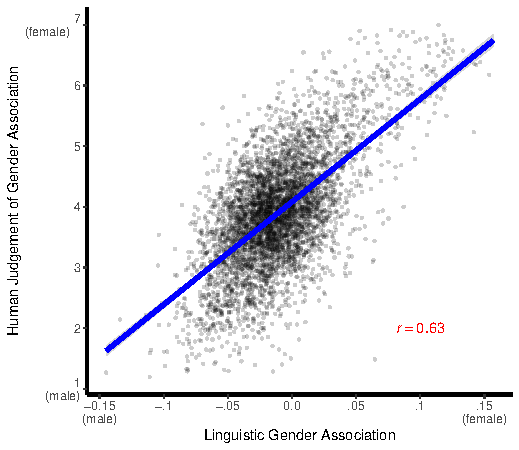
\includegraphics{../figs/fig1.pdf}
\caption{ Human judgments of word gender association as
a function of gender association from the Subtitle-trained embedding model
(\emph{r}(4669) = 0.63 {[}0.61, 0.65{]}; \emph{p} \textless{} .001; {\emph n} = 4,671; Study 1a). Each point corresponds to a word. Larger numbers indicate
stronger association with females (note that this differs from the
design of the rating task, but is changed here for consistency with
other plots). Blue line shows linear fit and the error band indicates
standard error.}
\end{figure}


\begin{figure*}
\centering
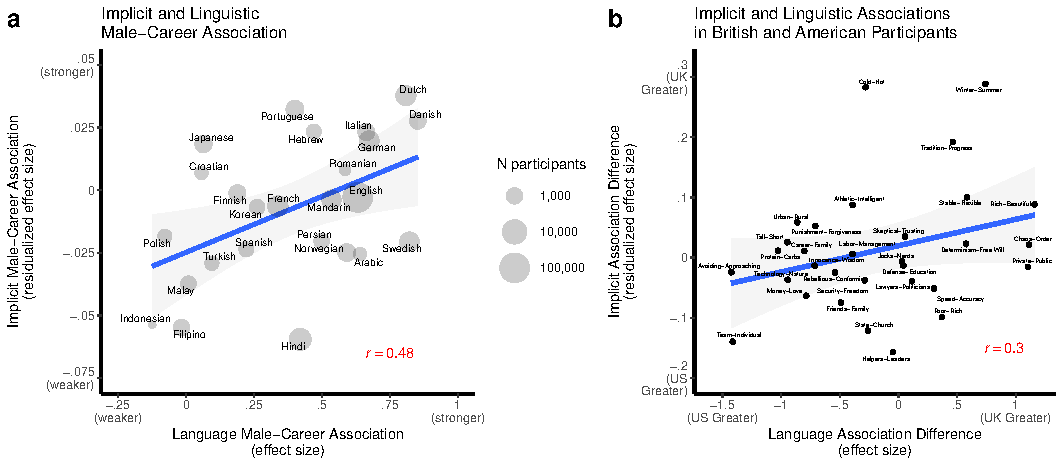
\includegraphics{../figs/fig2.pdf}
\caption{ ({\it a})  Implicit male-career association (adjusted for participants' age, gender, and congruent/incongruent block order) as a function of the linguistic male-career association derived from word-embeddings (\emph{r}(23) = 0.48 {[}0.11, 0.74{]}; \emph{p} = 0.01; \emph{n} = 25; Study 1b). Each point corresponds to a language. The size of the point is proportional to the number of participants who come from the country in which the language is dominant ({\it N} total = 656,636 participants). Linguistic associations are estimated from models trained on text in each language from the Wikipedia corpus. Larger values indicate a greater tendency to associate men with the concept of career and women with the concept of family. ({\it b}) Difference (UK minus US) in implicit association versus linguistic association for 31 IAT types (Study 1c). Error bands indicate standard error of the linear model
estimate.}
\end{figure*}

\begin{figure*}
\centering
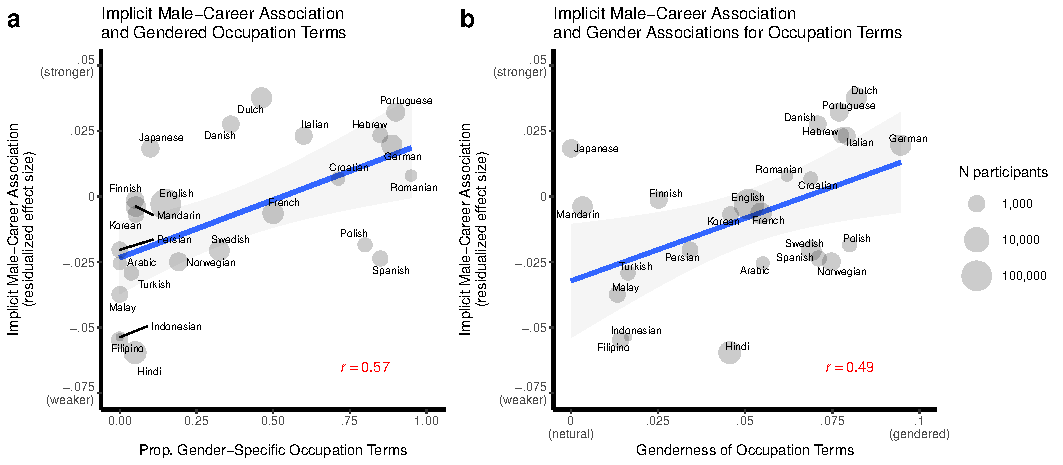
\includegraphics{../figs/fig3.pdf}
\caption{ Implicit male-career association (adjusted for participant age,
gender, and block order) as a function of the proportion of gender-specific labels for the set of words referring to occupations ({\it a}, left; \emph{r}(23) = 0.57 {[}0.22, 0.79{]}; \emph{p} = 0.003; \emph{n} = 25) and  mean gender association of words
referring to occupations from word embeddings trained on the Wikipedia corpus ({\it b}, right; \emph{r}(23) = 0.49 {[}0.11, 0.74{]}; \emph{p} = 0.01). Each point corresponds to a language, with the size of the point corresponding to the number of participants
speaking that language ({\it N} total = 656,636 participants). Error bands indicate standard error of the
linear model estimate.}
\end{figure*}


\newpage







\end{document}